\documentclass[a4paper,14pt,oneside,openany]{memoir}
\usepackage{coursework}
    
% Информация для титульного листа и листа задания
% Следует заполнить актуальными данными

% Кафедра, на которой читается дисциплина
\setdepartment{Электронно-вычислительные машины и системы}

% Инициалы и фамилия заведующего кафедрой
\setdepartmentchairname{А.Е.~Андреев}

% Полное название дисциплины
\setsubject{Системы обработки больших данных}

% Название темы курсовой работы
\settheme{Исследование датасета рейтинга недвижимости в Англии с использованием фреймворка Apache Spark}

% Фамилия Имя Отчество студента
\setstudentname{Ефременков Илья Евгеньевич}

% Инициалы и фамилия студента
\setstudentinitials{И.Е.~Ефременков}

% Учебная группа студента
\setgroupname{САПР-1.3}

% Инициалы и фамилия преподавателя, проверяющего курсовую работу
\setadvisorname{П.Д.~Кравченя}


\begin{document}

\maketitlepage % Создаем титульный лист

\renewcommand{\contentsname}{Содержание}
\tableofcontents*
\addtocontents{toc}{\vspace{1\baselineskip}}
\clearpage

\justifying
\chapter*{Введение}
\addcontentsline{toc}{chapter}{\MakeUppercase{Введение}}
\vspace{\baselineskip}

% Содержание введения
%
Во введении сначала дается краткая характеристика области, в которой выполнена работа (1 -- 3 предложения). Затем обосновывается актуальность работы.

Данная работа выполнена в среде Appache Spark - - это мощный open-source фреймворк для обработки больших данных, который применяется в различных областях:
В целом, область применения Apache Spark очень широка и зависит от потребностей конкретной организации или проекта.

Далее идут фразы, которые лучше повторить дословно:

В связи с этим целью данной работы являлось ... (цель должна быть одна). ?????????????(в двух лабах их несколько)

Для достижения поставленной цели решались следующие задачи:
\begin{enumerate}
\item Познакомиться с понятием «большие данные» и способами их обработки.
\item Познакомиться с инструментом Apache Spark и возможностями, которые он предоставляет для обработки больших данных.
\item Получить представление об инструментах экосистемы Hadoop: HDFS и YARN.
\item Поработать с табличным форматом для больших данных Apache Iceberg.
\item Получить навыки выполнения разведочного анализа данных использованием pyspark.
\end{enumerate}


В конце введения следует добавить описание структуры курсовой работы. Например:
\par В первом разделе рассмотрена более подробно постановка задачи разведовочного анализа датасета с использование фреймворка Apache Spark и библиотеки SparkML
\par Во втором разделе расмотрены более подробно задачи линейной регрессии и бинарной классификации
\par... В третьем разделе ???????????????
\par ... В заключении работы сформулированы общие выводы ???????

% Здесь пишется содержание первой главы
%
\chapter{\MakeUppercase{Разведочный анализ данных с использованием PySpark}}\label{ch:first}
\section{Постановка задачи разведочного анализа}\vspace{\baselineskip}

Разведочный анализ датасета - это первый этап в процессе анализа данных, который состоит из нескольких шагов. Цель этого этапа - получить общее представление о данных и их характеристиках, чтобы понять, какие методы анализа могут быть применены.

Основные цели разведочного анализа датасета включают:
\begin{enumerate}
\item Определение структуры данных: Разведочный анализ помогает определить, как выглядит ваш датасет – сколько столбцов (признаков) и строк (данных), какие типы данных используются (числовые, категориальные и т.д.).
\item Понимание распределения данных: Этот этап включает в себя проверку на наличие отсутствующих значений, выбросов или аномалий в данных.
\item Изучение основных характеристик данных: Определение среднего значения, моды, медианы и стандартного отклонения для числовых признаков; подсчет количества уникальных категорий для категориальных признаков.
\item Выявление взаимосвязей между переменными: Этот этап помогает понять, какие признаки могут влиять на другие в вашем датасете.
\item Визуализация данных: Построение графиков и диаграмм для наглядного представления данных и их распределения.
\end{enumerate}
Все эти шаги важны для того, чтобы понять ваши данные и выбрать правильные методы для дальнейшего анализа или машинного обучения.


\vspace{\baselineskip}\section{Описание датасета}\vspace{\baselineskip}

%Здесь требуется описать выбранный датасет, привести ссылку на него, охарактеризовать его тематику, объем, количество признаков. Вкратце нужно описать признаки датасета (допускается описывать не все признаки, а только те, которые используются в исследовании).
%Также, можно сослаться на источники, например, в \cite{karau2015spark, koirala2020pyspark, white2013hadoop, Tekdogan2022} рассматривается материал об ... Часть информации можно оформить в виде таблицы, но избегайте слишком длинных таблиц. На каждую таблицу должна быть ссылка в тексте, как, например, на таблицу \ref{tab:features}, в которой приведен пример описания признаков.

В приведенном датасете рассматриваются квартиры и их атрибуты для расчёта платы, такие как: площадь квартиры, её тип, использованное количество энергии, расход горячей воды и т.д. Таким образом из всех имеющихся признаков определяется рейтинг квартиры. Сам датасет весит более 20 Гб, но для работы с ним нам пришлось его обрезать до 5 Гб \cite{https://www.kaggle.com/datasets/tyagia1/epcratingsenglandjuly203}. Выбраны определенные 10 столбцов признаков для выполнения разведочного анализа.

\begin{table}[]
    \centering
    \begin{tabularx}{\textwidth}{|X|X|}
        \hline
        \multicolumn{1}{|c|}{Признак}  & \multicolumn{1}{c|}{Расшифровка признака}   \\ \hhline{|=|=|}
        LMK\_KEY					& Первичный ключ      \\ \hline
        ADDRESS					& Адрес                       \\ \hline
        CURRENT\_ENERGY\_EFFICIENCY	&  Эффективность энергии      \\ \hline
        PROPERTY\_TYPE                             	& Тип квартиры                       \\ \hline
        INSPECTION\_DATE                          	& Дата инспекции      \\ \hline
        HEATING\_COST\_CURRENT             	& Затраты на обогрев                       \\ \hline
        HOT\_WATER\_COST\_CURRENT	& Затраты на горячую воду      \\ \hline
        TOTAL\_FLOOR\_AREA                       	& Площадь                       \\ \hline
        NUMBER\_HABITABLE\_ROOMS       	& Количество обитаемых комнат     \\ \hline
        NUMBER\_HEATED\_ROOMS          	& Количество комнат с подогревом                       \\ \hline
    \end{tabularx}
    \caption{Таблица признаков}
    \label{tab:features}
\end{table}

\vspace{\baselineskip}\section{Определение пропущенных значений}\vspace{\baselineskip}

%Обратите внимание, что приведенная здесь структура раздела не является жестким требованием, а служит примером оформления. При необходимости, её можно корректировать в разумных пределах.
%При необходимости можно вставить рисунок и сослаться на него: на рисунке \ref{fig:HadoopEcoSystem} приведена иллюстрация экосистемы Hadoop. Обратите внимание, что таблицы и рисунки являются <<плавающими>> объектами: они могут располагаться не в месте их непосредственного объявления, а в некоторой близости от него.
%\begin{figure}
 %   \centering
 %   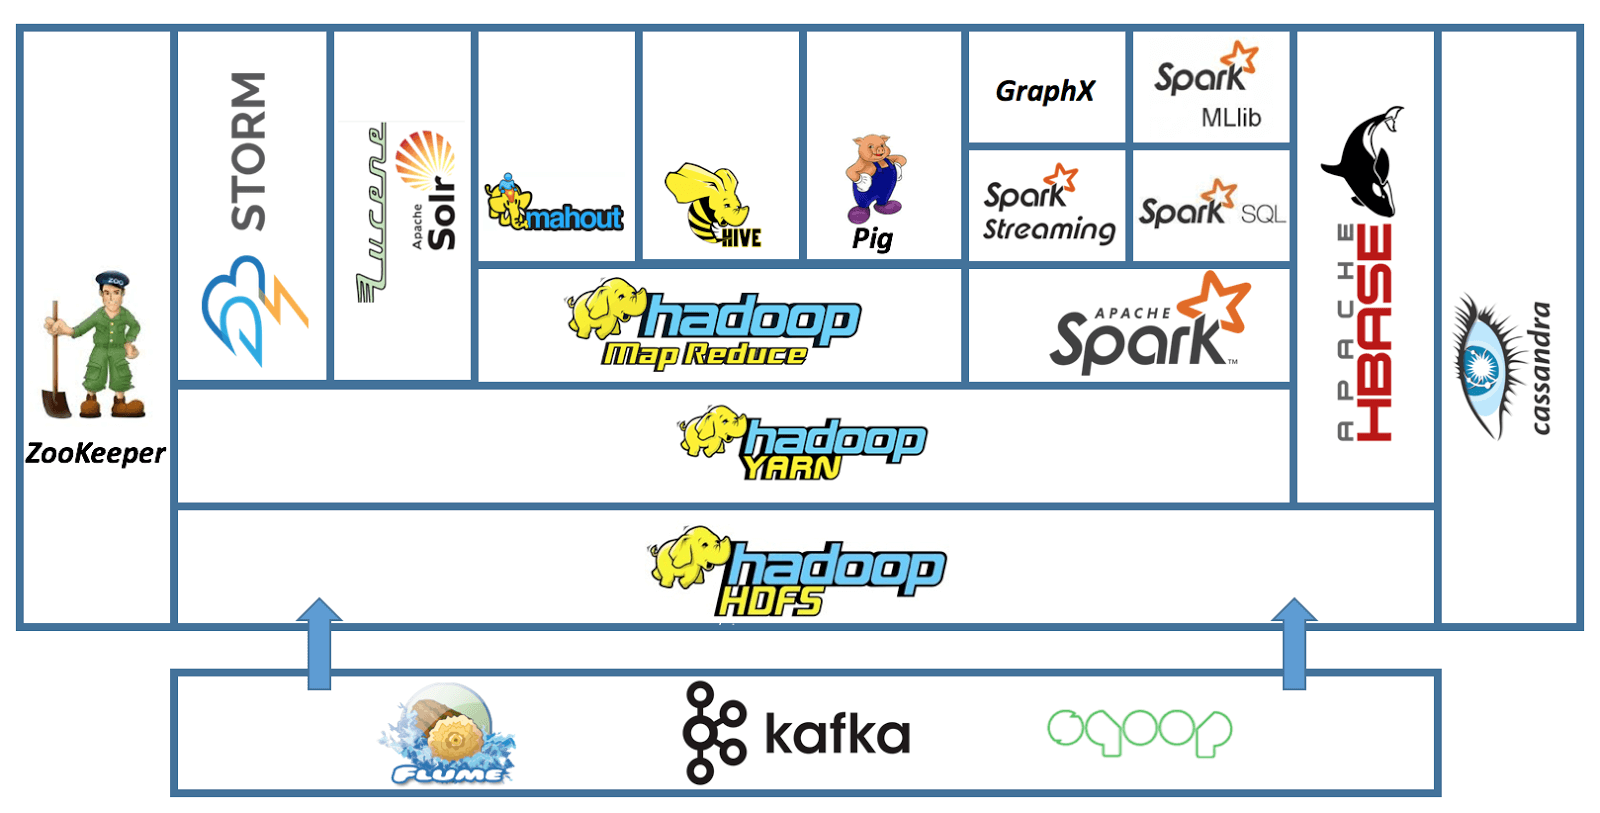
\includegraphics[width=\textwidth]{Content/Images/HadoopEcoSystem.png}
%    \caption{Иллюстрация экосистемы Hadoop}
%    \label{fig:HadoopEcoSystem}
%\end{figure}

%Также, вот пример списка:
При анализе мы предполагали, где  могут встречаться пропущеннные значения. С помощью команды count\_nulls мы определяли количества пропущенных значений в том или ином столбце. Ниже приведен список признаков, где пропущенные значения были недопустимы

А здесь -- аналогичный нумерованный список:

\begin{enumerate}
    \item ADDRESS3;
    \item HEATING\_COST\_CURRENT;
    \item NUMBER\_HABITABLE\_ROOMS
    \item NUMBER\_HEATED\_ROOMS
\end{enumerate}
\par После определения количества пропущенных значений мы работали с этими критериями мы их обрабатывали разными способами.
\par У ADDRESS3 более 90\% значений пропущены, этот столбец был удален в целях упрощения работы с датасетом.
\begin{code}
df = df.drop("ADDRESS3")
df.show()
\end{code}
В аналогичном случае можно было бы заменить пропущенные значения на значение Unknown
\begin{code}
df = df.fillna({"PROPERTY\_TYPE": "Unknown"})
count\_nulls(data=df, column\_name="PROPERTY\_TYPE")
\end{code}

\par В столбце HEATING\_COST\_CURRENT было пропущенно значений меньше половины, значит, можно попытаться обработать эти данные. Была создана функция позволяющая рассчитывать статистические показатели данных в столбцах и строить диаграмму "ящик с усами" для оценки наличия выбросов: "plot\_boxplots".
\begin{figure}
    \centering
    \includegraphics[width=\textwidth]{Content/Images/vibroses.png}
    \caption{Выбросы в HEATING\_COST\_CURRENT}
    \label{fig:VHCC}
\end{figure}
В результате получился boxplot с сильными выбросами в нескольких точках. Удалим строки, их содержащие, и убедимся, что потеряна небольшая часть данных и заменим пропуски средним значением признака.
\begin{code}
df.filter(col("HEATING\_COST\_CURRENT") > 8000).count()
df = df.filter(col("HEATING\_COST\_CURRENT") < 8000)
mean\_cost = df.select(mean(col("HEATING\_COST\_CURRENT"))).collect()[0][0]
mean\_cost
df = df.fillna({"HEATING\_COST\_CURRENT": mean\_cost})
\end{code}

\par В столбцах NUMBER\_HABITABLE\_ROOMS и NUMBER\_HEATED\_ROOMS содержатся пропущенные значения с типом float, заменим их на значения 0.0

\begin{code}
df = df.fillna({"NUMBER\_HABITABLE\_ROOMS": 0.0})
df = df.fillna({"NUMBER\_HEATED\_ROOMS": 0.0})
\end{code}

%%А вот формула, которая связывает между собой синус, косинус и тангенс.

%\begin{equation}
%    \label{eq:formula}
%    \tg \alpha = \frac{\sin \alpha}{\cos \alpha}.
%\end{equation}

%Ну, и ссылка на неё: формула (\ref{eq:formula}) выражает связь тригонометрических функций.

\vspace{\baselineskip}\section{Расчет корреляции между количественными признаками}\vspace{\baselineskip}

Рассчет корреляции между количественными признаками — это процесс, который позволяет определить степень и направление взаимосвязи между двумя или более переменными. Корреляция отражает насколько часто значения одной переменной изменяются вместе с изменениями в другой переменной.


Существует два основных типа корреляции:

\begin{enumerate}
\item Позитивная корреляция: Это ситуация, когда значения двух переменных меняются в одно и то же направление. Например, если при увеличении одной переменной (например, времени) увеличивается и другая (например, расстояние), это будет показывать положительную корреляцию.
\item Негативная корреляция: Это ситуация, когда значения двух переменных меняются в противоположных направлениях. Например, если при увеличении одной переменной (например, времени) уменьшается другая (например, расстояние), это будет показывать негативную корреляцию.
\end{enumerate}

\par Рассчитать корреляцию между количественными признаками можно с помощью различных статистических методов. Наиболее распространенным из них является коэффициент корреляции Пирсона, который показывает степень и направление линейной связи между двумя переменными.

Коэффициент корреляции Пирсона (r) вычисляется по формуле:

$$r = \frac{\sum_{i=1}^{n}(x_i - \bar{x})(y_i - \bar{y})}{\sqrt{\sum_{i=1}^{n}(x_i - \bar{x})^2 \sum_{i=1}^{n}(y_i - \bar{y})^2}}$$


В большинстве случаев используется коэффициент корреляции Пирсона для измерения линейной связи между двумя количественными признаками. Коэффициент Пирсона, обозначенный как r, варьируется от -1 до 1:
\begin{enumerate}
\item Если r близок к 1, то связь между переменными очень сильная и положительная.
\item Если r близок к -1, то связь между переменными очень сильная и негативная.
\item Если r близок к 0, то между переменными нет линейной связи.
\end{enumerate}

Важно отметить, что корреляция не говорит о причине и последствии между двумя переменными; она просто показывает, насколько сильно значения одной переменной изменяются в зависимости от значений другой.

\par Корреляционные коэффициенты часто используются для анализа и визуализации данных, чтобы определить взаимосвязь между различными признаками. Они могут помочь в выборе переменных для моделей машинного обучения или в выявлении закономерностей в данных.

Код расчёта:
\begin{code}
def compute_and_visualize_correlation_matrix(data: DataFrame, 
                                             columns: list[str]) -> None:
    """
    Вычисляет и визуализирует корреляционную матрицу для указанных 
    колонок в DataFrame PySpark.

    Args:
        df (DataFrame): DataFrame PySpark.
        columns (list[str]): Список колонок для вычисления корреляции.

    Returns:
        None
    """
    # Вычисление корреляционной матрицы
    corr_matrix = {}
    for col1 in columns:
        corr_matrix[col1] = {}
        for col2 in columns:
            corr_value = data.select(corr(col1, col2)).collect()[0][0]
            corr_matrix[col1][col2] = corr_value

    # Преобразование корреляционной матрицы в DataFrame Pandas для визуализации
    corr_matrix_pd = pd.DataFrame(corr_matrix)

    # Построение и визуализация корреляционной матрицы
    plt.figure(figsize=(10, 8))
    sns.heatmap(corr_matrix_pd, annot=True, cmap='coolwarm', linewidths=0.5)
    plt.title('Correlation Matrix')
    plt.show()
\end{code}

%Здесь можно продемонстрировать пример включения фрагмента кода в текст работы. И заодно добавить еще пару ссылок \cite{spark2022official, zaharia2021lakehouse}.
%\begin{code}
%import matplotlib.pyplot as plt
%import numpy as np
%x = np.linspace(0, 10, 100)
%y = np.sin(x)
%plt.figure(figsize=(10, 6))
%plt.plot(x, y, label='sin(x)', color='blue', linewidth=2)
%plt.title('График функции sin(x)', fontsize=16)
%plt.xlabel('x', fontsize=14)
%plt.ylabel('sin(x)', fontsize=14)
%plt.legend()
%plt.grid(True)
%plt.show()    
%\end{code}

%Здесь продолжается текст. Не забывайте, что фрагмент кода не должен превышать половины страницы -- затем должен следовать текст.

\vspace{\baselineskip}\section{Выводы}\vspace{\baselineskip}

В результате полученной работы была разработана корреляционная матрица, демонстрирующая наличие корреляции между количественными признаками.

\begin{figure}
    \centering
    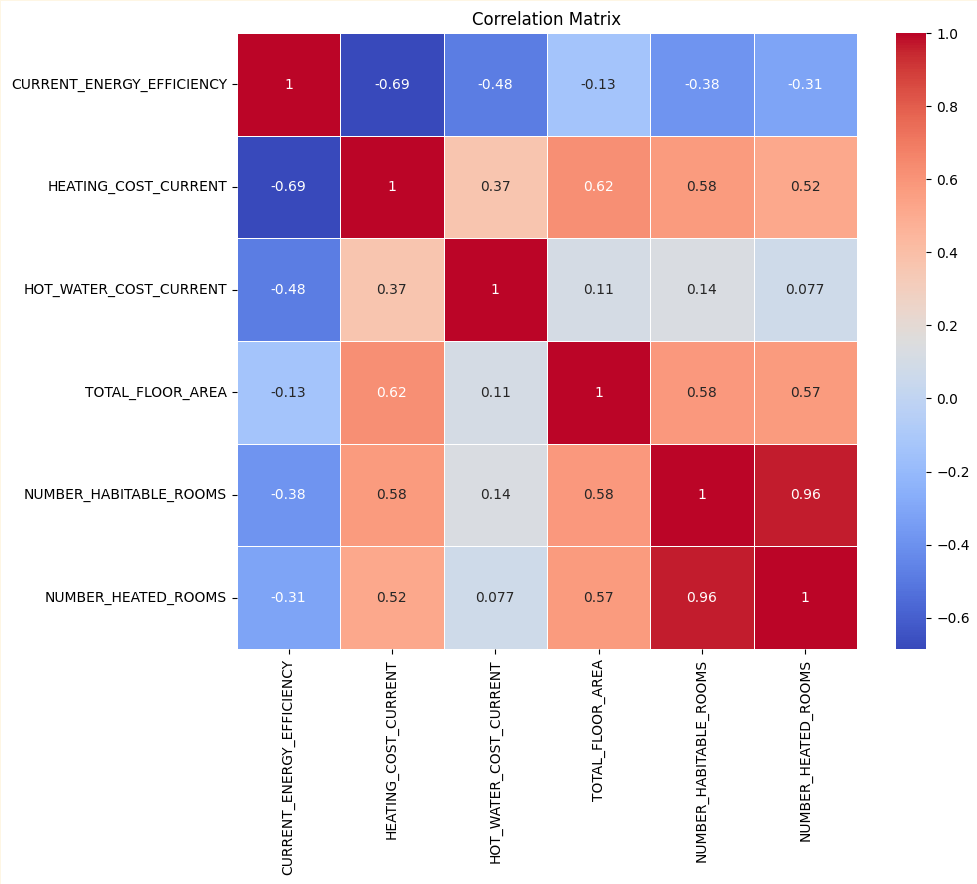
\includegraphics[width=\textwidth]{Content/Images/CorMatrixOfDataset.png}
    \caption{Корреляционная матрица датасета}
    \label{fig:CorMatrixOfDataset}
\end{figure}

Здесь наблюдается наибольшая зависимость  обитаемых и обогреваемых комнат от площади самой квартиры.


% Здесь пишется содержание второй главы
%
\chapter{\MakeUppercase{Машинное обучение на больших данных}}\label{ch:second}

\vspace{\baselineskip}
В этой главе подробно рассматриваются задачи линейной регрессии и бинарной классификации больших данных.
\vspace{\baselineskip}

\section{Задача регресии}
\subsection{Постановка задачи регрессии}\vspace{\baselineskip}

Постановка задачи линейной регрессии заключается в построении математической модели, которая позволяет предсказывать значение зависимой переменной на основе независимых переменных. Целью является минимизация ошибок и нахождение коэффициентов, которые обеспечивают наиболее точные прогнозы. В данном датасете мы, исходя из разведочного анализа, выяснили предсказываем значение зависимого столбца TOTAL\_FLOOR\_AREA. Также нужно рассчитать оценку качества модели.

Для датасета, заданного представленными колонками, требуется построить модель линейной регрессии для оценки **Площадь квартиры** по всем колличественным и категориальным признакам. 

Для оценки качества обучения следует использовать метрики $RMSE$ и $R^2$.

\vspace{\baselineskip}\subsection{Решение задачи регрессии}\vspace{\baselineskip}

\par Подготовка и кодирование признаков.
\par Для корректной работы трансформеров преобразуем столбцы `HEATING\_COST\_CURRENT`, `HOT\_WATER\_COST\_CURRENT`, `NUMBER\_HABITABLE\_ROOMS`, `NUMBER\_HEATED\_ROOMS` к типу `DoubleType`.
\begin{code}
df = df.withColumn("HEATING_COST_CURRENT", col("HEATING_COST_CURRENT").cast(DoubleType()))
df = df.withColumn("HOT_WATER_COST_CURRENT", col("HOT_WATER_COST_CURRENT").cast(DoubleType()))
df = df.withColumn("NUMBER_HABITABLE_ROOMS", col("NUMBER_HABITABLE_ROOMS").cast(DoubleType()))
df = df.withColumn("NUMBER_HEATED_ROOMS", col("NUMBER_HEATED_ROOMS").cast(DoubleType()))
\end{code}

Отделим от датасета некоторую часть объёмом примерно 1000 строк, и сохраним её на диске как локальный `csv`-файл. Он понадобится в следующей лабораторной работе.
\begin{code}
def save_sample_to_csv(data: DataFrame, file_path: str, 
                       sample_size: int = 1000) -> DataFrame:
\end{code}

Определяем путь для сохранения `csv`-файла.
\begin{code}
path = "/home/user6/Efremenkov_directory/dataset/data/epc_cut_reg.csv"
df = save_sample_to_csv(data=df, file_path=path, sample_size=1000)
\end{code}

Оцениваем, сколько строк в датасете осталось.
\begin{code}
df.count()
\end{code}

Разделим датасет на обучающую и тестовую выборки.
\begin{code}
train_df, test_df = df.randomSplit([0.8, 0.2])
\end{code}

Понятно, что **ключ и адрес** квартиры не оказывает влияния на тип недвижимости. Использовать его в модели нет смысла.
Остальные признаки сгруппируем по их типу:

* **Категориальные** признаки не содержат большого количества категорий, закодируем их `one-hot`-кодировкой.
* **Бинарные** признаки представлены значениями `true` / `false`, которые могут быть интерпретированы как единица и нуль. Поэтому, в кодировании не нуждаются.
* **Количественные** признаки нужно нормализовать / стандартизировать, перед тем, как передавать их в модель.

\begin{code}
categorical_features = [ "PROPERTY_TYPE" ]
numeric_features = [
    "CURRENT_ENERGY_EFFICIENCY", "HEATING_COST_CURRENT", "HOT_WATER_COST_CURRENT", "NUMBER_HABITABLE_ROOMS", "NUMBER_HEATED_ROOMS"
]
\end{code}

Создадим конвейер обработки данных, включающий модель линейной регрессии.
\begin{code}
def create_pipeline(categorical_features: list[str], 
                    numeric_features: list[str], 
                    #binary_features: list[str], binarized_col: str, 
                    #threshold: float, 
                    label_col: str, max_iter: int) -> Pipeline: ... Смотри в приложении...
                    
pipeline = create_pipeline(categorical_features=categorical_features,
                           numeric_features=numeric_features,
                           #binary_features=binary_features,
                           label_col="TOTAL_FLOOR_AREA",
                           max_iter=15)
\end{code}


\par Обучение модели.
Выполним **подбор гиперпараметров** модели линейной регрессии с помощью кросс-валидации на сетке. 
Создаем сетку параметров для кросс-валидации, получив объект `LinearRegression` из конвейера.
Создаем экземпляр `RegressionEvaluator` для оценки модели.
Создаем объект `CrossValidator`.
\begin{code}
param_grid = ParamGridBuilder() \
    .addGrid(pipeline.getStages()[-1].regParam, [0.01, 0.1, 1.0]) \
    .addGrid(pipeline.getStages()[-1].elasticNetParam, [0.0, 0.5, 1.0]) \
    .build()
    
cv_evaluator = RegressionEvaluator(labelCol="TOTAL_FLOOR_AREA",
                                   predictionCol="prediction",
                                   metricName="rmse")
                                   
cross_validator = CrossValidator(estimator=pipeline,
                                 estimatorParamMaps=param_grid,
                                 evaluator=cv_evaluator,
                                 numFolds=5)
\end{code}

Обучаем модель конвейера с использованием кросс-валидации.
\begin{code}
cv_model = cross_validator.fit(train_df)
\end{code}

Выведем параметры **лучшей** модели, определенной в ходе кросс-валидации.
\begin{code}
def get_best_model_params(cv_model: CrossValidatorModel) -> dict[str, float]: ...приложение...
for key, value in get_best_model_params(cv_model=cv_model).items():
    print(f"{key}: {value}")
\end{code}



\vspace{\baselineskip}\subsection{Анализ полученных результатов}\vspace{\baselineskip}

Визуализируем изменение ошибки модели в ходе обучения и рассчитаем метрики на обучающем датасете.
\begin{code}
def plot_training_summary(cv_model: DataFrame) -> None: ... Приложение...
plot_training_summary(cv_model)
\end{code}

\begin{figure}
    \centering
    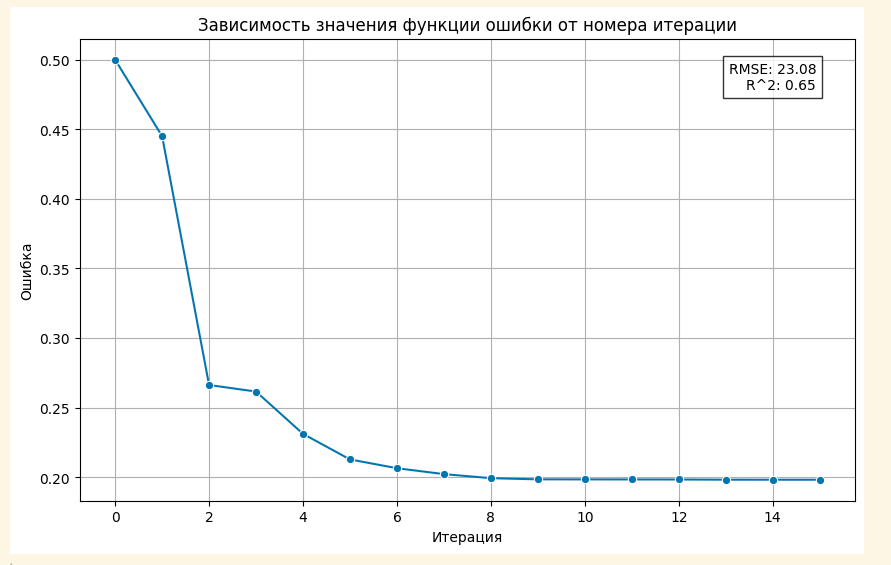
\includegraphics[width=\textwidth]{Content/Images/Zavisimost.png}
    %\caption{Корреляционная матрица датасета}
    \label{fig:ZZFOONI}
\end{figure}

\par Проверка обобщающей способности модели
Выполним предсказания на тестовой выборке. 
Перегруппируем колонки датафрейма, переставив столбец с площадью квартиры в конец, чтобы его значения было удобно сравнивать с предсказанными.
\begin{code}
# Получаем датасет предсказаний
test_df_predictions = cv_model.transform(test_df)

# Извлекаем список колонок, устанавливаем цену на последнее место
right_columns_order = test_df_predictions.columns
right_columns_order.remove("TOTAL_FLOOR_AREA")
right_columns_order.append("TOTAL_FLOOR_AREA")

# Изменяем последовательность колонок и выводим датафрейм
test_df_predictions = test_df_predictions.select(*right_columns_order)
test_df_predictions.show()
\end{code}

Создадим функцию оценки модели: расчета метрик для некоторого датасета, как правило, тестового.
\begin{code}
def evaluate_model(data: DataFrame, metric_name: str) -> float:
\end{code}

Оценим модель на тестовой выборке.
\begin{code}
test_rmse = evaluate_model(test_df_predictions, "rmse")
test_r2 = evaluate_model(test_df_predictions, "r2")

print(f"RMSE on test data: {test_rmse:.2f}")
print(f"R^2 on test data: {test_r2:.2f}")
\end{code}

Результат: 
\begin{enumerate}
\item RMSE on test data: 22.95
\item R\^2 on test data: 0.65
\end{enumerate}
Метрики весьма неплохие для данной модели.

\vspace{\baselineskip}\section{Задача бинарной классификации}

\par В данной части работы рассмотрены:
\begin{itemize}
\item подготовка признаков для рашения задачи **градиентного бустинга** на деревьях решений;
\item создание и обучение модели градиентного бустинга;
\item оценка качества модели.
\end{itemize}

\subsection{Постановка задачи бинарной классификации}\vspace{\baselineskip}

\par Постановка задачи бинарной классификации включает определение, какие данные будут использоваться для обучения модели, выбор метрик для оценки качества модели и определение целевой переменной.

\begin{enumerate}
\item Определение данных

\par Для построения модели необходимо иметь набор данных, который содержит:

\begin{enumerate}
\item Входные признаки (features): Эти данные используются для прогнозирования целевой переменной.
\item Целевая переменная (target variable): Эта переменная представляет собой класс, к которому относится каждый объект в наборе данных. В случае бинарной классификации это обычно два значения, например, 0 и 1.
\end{enumerate}

\item Выбор метрик для оценки качества модели

Для оценки качества модели на этапе тестирования используются различные метрики. Основные метрики в бинарной классификации:

\begin{enumerate}
\item Точность (Precision): Процент объектов, которые действительно принадлежат положительному классу и были корректно определены моделью. [ $Precision = \frac{TP}{TP + FP}$ ] Где ( TP ) — истинные положительные, а ( FP ) — ложные положительные.
\item Полнота (Recall): Процент объектов, которые действительно принадлежат положительному классу и были корректно определены моделью. [ $Recall = \frac{TP}{TP + FN}$ ] Где ( TP ) — истинные положительные, а ( FN ) — ложные отрицательные.
\item F1-мера: Среднее гармоническое точности и полноты. Это метрика, которая учитывает обе ошибки (FP и FN). [ $F1 = 2 \cdot \frac{Precision \cdot Recall}{Precision + Recall}$ ]
\item ROC-AUC (Area Under the Receiver Operating Characteristic Curve): Площадь под кривой ROC, которая показывает, как хорошо модель различает положительные и отрицательные классы при различных порогах вероятности.
\begin{enumerate}
\item Кривая ROC строится на основе значений вероятностей принадлежности положительному классу для всех объектов в наборе данных.
\end{enumerate}

\end{enumerate}

\item Определение целевой переменной
\end{enumerate}
Целевая переменная в бинарной классификации должна быть категориальной и иметь всего два уникальных значения, например, "0" и "1". Значения могут представлять собой различные классы или категории, такие как "заболевал" vs "не заболевал", "покупает" vs "не покупает".

Шаги построения модели
\begin{enumerate}
\item Подготовка данных:
	\begin{enumerate}
	\item Разделить данные на наборы для обучения и тестирования.
	\item Нормализовать или стандартизировать признаки.
	\item Обработать пропущенные значения (например, удалить строки с пропущенными значениями).
	\end{enumerate}
\item Выбор модели:
	\begin{enumerate}
	\item Выбрать подходящую модель бинарной классификации, например, логистическая регрессия, случайный лес или нейронную сеть.
	\end{enumerate}
\item Обучение модели:
	\begin{enumerate}
	\item Обучить модель на наборе данных для обучения.
	\end{enumerate}
\item Оценка качества модели:
	\begin{enumerate}
	\item Оценить качество модели на наборе данных для тестирования.
	\item Использовать выбранные метрики (точность, полнота, F1-мера, ROC-AUC) для оценки производительности модели.
	\end{enumerate}
\item Кросс-валидация:
	\begin{enumerate}
	\item Применить кросс-валидацию для улучшения надежности оценок качества модели.
	\end{enumerate}
\item Оптимизация параметров:
	\begin{enumerate}
	\item Оптимизировать параметры модели с помощью методов, таких как градиентный спуск или случайный поиск.
	\end{enumerate}
\item Интерпретация результатов:
	\begin{enumerate}
	\item Понять, какие признаки влияют на вероятность открытия нового счета.
	\item Делать выводы о том, насколько хорошо модель предсказывает целевую переменную.
	\end{enumerate}
\end{enumerate}

Для датасета, заданного представленными колонками, требуется построить модель градиентного бустинга на деревьях решений для оценки факта того, является ли автомобиль сертифицированным, по всем остальным признакам. 

Для оценки качества обучения следует использовать метрики `Precision` и `Recall`. Оценить максимально возможное значение точности при полноте не менее 60%.

\vspace{\baselineskip}\subsection{Решение задачи бинарной классификации}\vspace{\baselineskip}

\p Для корректной работы трансформеров преобразуем столбцы `HEATING\_COST\_CURRENT`, `HOT\_WATER\_COST\_CURRENT`, `NUMBER\_HABITABLE\_ROOMS`, `NUMBER\_HEATED\_ROOMS` к типу `DoubleType`, а столбец `TOTAL\_FLOOR\_AREA` сделаем бинаризируемым с преобразованием в `Double`

\begin{code}
df = df.withColumn("HEATING_COST_CURRENT", F.col("HEATING_COST_CURRENT").cast(DoubleType()))\n
df = df.withColumn("HOT_WATER_COST_CURRENT", F.col("HOT_WATER_COST_CURRENT").cast(DoubleType()))\n
df = df.withColumn("NUMBER_HABITABLE_ROOMS", F.col("NUMBER_HABITABLE_ROOMS").cast(DoubleType()))\n
df = df.withColumn("NUMBER_HEATED_ROOMS", F.col("NUMBER_HEATED_ROOMS").cast(DoubleType()))\n
\end{code}

\p Бинаризируем столбец TOTAL\_FLOOR\_AREA. Выполняется 1 раз

\begin{code}
udfValueToCategory = udf(valueToCategory, DoubleType())
df = df.withColumn("TOTAL_FLOOR_AREA", udfValueToCategory("TOTAL_FLOOR_AREA") )
\end{code}

\p Выполним **стратифицированное** разделение датасета на обучающую и тестовую выборки.

\begin{code}
def stratified_train_test_split(data: DataFrame, 
                                label_col: str,
                                ratio: float) -> tuple[DataFrame, DataFrame]:
    """
    Разделяет DataFrame на тренировочный и тестовый наборы с учетом стратификации.

    Args:
        data: Исходный DataFrame.
        label_col: Название столбца с меткой.
        ratio: Пропорция разделения данных.

    Returns:
        tuple[DataFrame, DataFrame]: Кортеж из тренировочного и тестового DataFrame.
    """
    # Проверяем корректность доли разделения
    assert (isinstance(ratio, float) and (0.0 <= ratio <= 1.0))
    
    # Формируем разделение для положительных и отрицательных объектов раздельно
    train_df_pos, test_df_pos = (data
                                 .filter(F.col(label_col) == 1)
                                 .randomSplit([ratio, 1 - ratio]))
    train_df_neg, test_df_neg = (data
                                 .filter(F.col(label_col) == 0)
                                 .randomSplit([ratio, 1 - ratio]))
    
    # Объединяем датафреймы
    return (train_df_pos.union(train_df_neg),
            test_df_pos.union(test_df_neg))
\end{code}


\p Выполним балансировку датасета с помощью `oversampling` - подбирает одинаковое количество 1 и 0. 

\begin{code}
def oversample(data: DataFrame, column: str) -> DataFrame:
    """
    Выполняет oversampling положительных классов в DataFrame.

    Args:
        data: Исходный DataFrame.
        column: Название столбца с меткой.

    Returns:
        DataFrame: Датафрейм с выполненным oversampling.
    """
    # Разделим датафрейм на положительные и отрицательные классы
    pos = data.filter(F.col(column) == 1.0)
    neg = data.filter(F.col(column) == 0.0)

    # Получим количество записей в каждом классе
    total_pos = pos.count()
    total_neg = neg.count()
    
    print(total_pos)
    print(total_neg)

    # Если количество положительных классов меньше отрицательных,
    # выполним oversampling
    if total_pos < total_neg:
        # Вычислим количество необходимых дубликатов
        num_duplicates = total_neg - total_pos
        print(num_duplicates)
        # Дублируем положительные записи
        oversampled_pos = pos.withColumn(
            "dummy",
            F.explode(
                F.array_repeat(F.lit(1),
                               num_duplicates // total_pos + 1)
            )
        ).drop("dummy")
        print(num_duplicates // total_pos + 1)
        # Объединим дублированные положительные записи с отрицательными
        balanced_df = neg.union(oversampled_pos)
    else:
        balanced_df = data

    return balanced_df
\end{code}

\p Понятно, что **ключ и адрес** квартиры не оказывает влияния на тип недвижимости. Использовать его в модели нет смысла.

Остальные признаки сгруппируем по их типу:

*\b{Категориальные} признаки не содержат большого количества категорий, закодируем их `one-hot`-кодировкой.
* \b{Бинарные} признаки представлены значениями `true` / `false`, которые могут быть интерпретированы как единица и нуль. Поэтому, в кодировании не нуждаются.
* \b{Количественные} признаки нужно нормализовать / стандартизировать, перед тем, как передавать их в модель.

\begin{code}
categorical_features = [ "PROPERTY_TYPE" ]
numeric_features = [
    "CURRENT_ENERGY_EFFICIENCY", "HEATING_COST_CURRENT", "HOT_WATER_COST_CURRENT", "NUMBER_HABITABLE_ROOMS", "NUMBER_HEATED_ROOMS"
]
\end{code}

\p Обучение модели
Выполним **подбор гиперпараметров** модели линейной регрессии с помощью кросс-валидации на сетке.
Создаем сетку параметров для кросс-валидации, получив объект `GBTClassifier` из конвейера.
Создаем экземпляр `BinaryClassificationEvaluator` для оценки модели.
Создаем объект `CrossValidator`.
Обучаем модель конвейера с использованием кросс-валидации.

\begin{code}
student_hdfs_folder = "Efremenkov_directory"
# Получаем имя пользователя
user_name = os.getenv("USER")

# Путь модели в HDFS
model_hdfs_path = f"hdfs:///user/{user_name}/{student_hdfs_folder}/models/GBT-model"

# Сохраняем модель конвейера в HDFS
try:
    cv_model.bestModel.save(model_hdfs_path)
    print(f"Модель успешно сохранена в \"{model_hdfs_path}\"")
except Exception as e:
    print(f"Ошибка при сохранении модели: {e}")
\end{code}

\p Выведем параметры **лучшей** модели, определенной в ходе кросс-валидации.

\begin{code}
def get_best_model_params(cv_model: CrossValidatorModel) -> dict[str, float]:
    """
    Получает параметры лучшей модели из объекта CrossValidatorModel.

    Args:
        cv_model: Объект CrossValidatorModel, содержащий лучшую модель.

    Returns:
        Dict[str, float]: Параметры лучшей модели.
    """
    best_model = cv_model.bestModel
    best_params = {
        "maxDepth": best_model.stages[-1].getMaxDepth(),
        "stepSize": best_model.stages[-1].getStepSize(),
        "maxIter": best_model.stages[-1].getMaxIter()
    }
    return best_params
\end{code}

\begin{code}
for key, value in get_best_model_params(cv_model=cv_model).items():
    print(f"{key}: {value}")
\end{code}

Результат:
\begin{enumerate}
\item maxDepth: 5
\item stepSize: 0.01
\item maxIter: 30
\end{enumerate}

\p Анализ обученной модели
\p Рассчитаем метрики на тестовом датасете.

\begin{code}
# Получаем датасет предсказаний
test_df_predictions = cv_model.transform(test_df)

# Извлекаем список колонок, устанавливаем цену на последнее место
right_columns_order = test_df_predictions.columns
right_columns_order.remove("TOTAL_FLOOR_AREA")
right_columns_order.append("TOTAL_FLOOR_AREA")

# Изменяем последовательность колонок и выводим датафрейм
test_df_predictions = test_df_predictions.select(*right_columns_order)
\end{code}

\begin{code}
def evaluate_model(data: DataFrame, 
                   label_col: str) -> dict[str, float]:
    """
    Оценивает модель с использованием метрик точности, полноты и F1-score.

    Args:
        data: DataFrame, содержащий предсказания и фактические метки.
        label_col: Название колонки с меткой.

    Returns:
        dict[str, float]: Словарь с метриками точности, полноты и F1-score.
    """
    # Вычисляем TP, FP, FN
    tp = data.filter((F.col(label_col) == 1) &
                     (F.col("prediction") == 1)).count()
    fp = data.filter((F.col(label_col) == 0) &
                     (F.col("prediction") == 1)).count()
    fn = data.filter((F.col(label_col) == 1) &
                     (F.col("prediction") == 0)).count()

    # Вычисляем метрики
    precision = tp / (tp + fp) if (tp + fp) > 0 else 0
    recall = tp / (tp + fn) if (tp + fn) > 0 else 0
    f1 = (2 * (precision * recall) / (precision + recall)
        if (precision + recall) > 0 else 0)

    # Возвращаем словарь с метриками
    return {
        "precision": precision,
        "recall": recall,
        "f1": f1
    }
\end{code}

\begin{code}
metrics = evaluate_model(test_df_predictions, "TOTAL_FLOOR_AREA")
print(f"Metrics: {metrics}")
\end{code}

\p Результат Metrics: 
\begin{enumerate}
\item 'precision': 0.859179580674567 
\item 'recall': 0.7177807853154796 
\item 'f1': 0.7821408926234328
\end{enumerate}

\p Наблюдаем довольно высокую точность при высокой полноте. Попробуем подобрать `threshold`, чтобы максимизировать точность, но при этом удерживать полноту на заданном в постановке задачи уровне.
Сначала рассчитаем `AUC ROC`, визуализируем `ROC` и `PR`-кривые и оценим ситуацию.

\begin{figure}
    \centering
    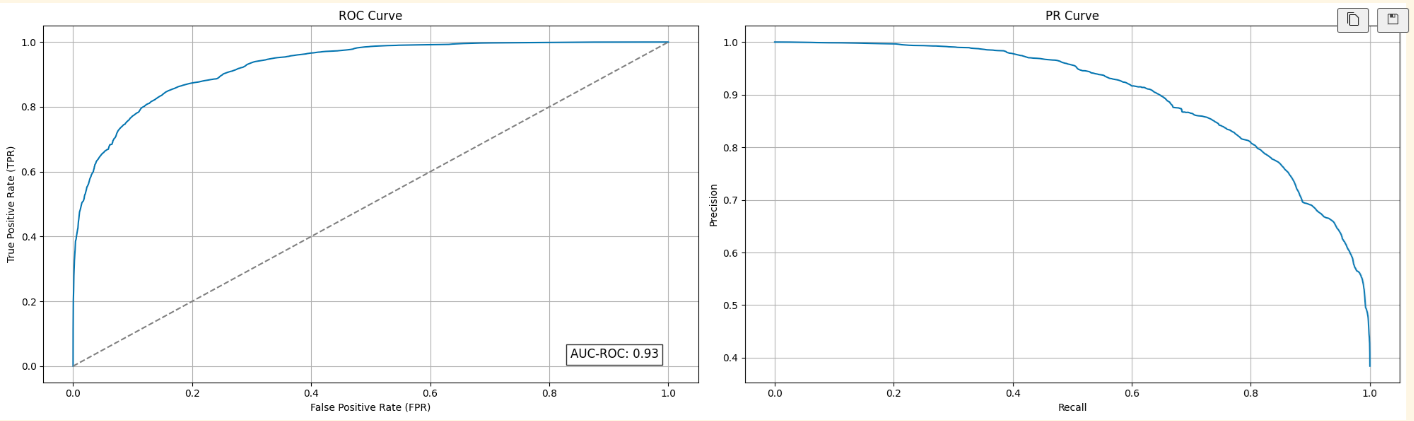
\includegraphics[width=\textwidth]{Content/Images/AUC_ROC.png}
    %\caption{Корреляционная матрица датасета}
    \label{fig:ZZFOONI}
\end{figure}

\vspace{\baselineskip}\subsection{Анализ полученных результатов}\vspace{\baselineskip}

\par Определим вероятность -- границу разделения, при которой `Recall` не меньше 60\%.
\begin{code}
threshold_probability = pd_dataframe[pd_dataframe['TPR'] >= 0.60]['probability'].max()
print(f"Вероятность -- граница разделения, при которой TPR не меньше 60\%: {threshold_probability:.2f}")
\end{code}
Вероятность -- граница разделения, при которой TPR не меньше 60\%: 0.70

\par Рассчитаем метрики на тестовом датасете повторно, с учетом вычисленного `threshold` для вероятности.
\begin{code}
cv_model.bestModel.stages[-1].setThresholds([1 - threshold_probability, 
                                             threshold_probability])
test_df_predictions = cv_model.transform(test_df)
metrics = evaluate_model(test_df_predictions, "TOTAL_FLOOR_AREA")
print(f"Metrics: {metrics}")
\end{code}
Результат Metrics: 
\begin{enumerate}
\item 'precision': 0.9164163632014035, 
\item 'recall': 0.6001314226281914, 
\item 'f1': 0.7252923526797572}
\end{enumerate}

\vspace{\baselineskip}\section{Выводы}\vspace{\baselineskip}

\par Обученная модель обладает очень хорошим качеством и не требует его дальнейшего улучшения.


% Здесь пишется содержание третьей главы
%


% Здесь пишется содержание четвёртой главы
%


\chapter*{Заключение}
\addcontentsline{toc}{chapter}{\MakeUppercase{Заключение}}
\vspace{\baselineskip}

% Здесь пишется заключение по работе
%
В заключении коротко приводятся и анализируются полученные результаты, предлагаются дальнейшие направления развития темы.

\clearpage

\printbibliography

%%% Настройки для приложений
\appendix

% Оформление заголовков приложений ближе к ГОСТ:
\renewcommand*{\printchaptername}{\MakeUppercase{\appendixname}}
\renewcommand*{\afterchapternum}{\centering\par\nobreak\vskip \midchapskip}
\renewcommand*{\printchapternum}{\chapnumfont \thechapter}
\renewcommand\thechapter{\Asbuk{chapter}}
\renewcommand*{\printchaptertitle}[1]{\chaptitlefont #1}

% Здесь пишется содержание приложений
%
\chapter{Пример листинга программного кода}\label{app:A}\vspace{\baselineskip}

Здесь можно привести полный листинг кода программы или модуля.

\begin{code}
import matplotlib.pyplot as plt
import numpy as np

# Данные для графика
x = np.linspace(0, 10, 100)
y = np.sin(x)

# Создание графика
plt.figure(figsize=(10, 6))

plt.plot(x, y, label='sin(x)', color='blue', linewidth=2)

# Настройка графика
plt.title('График функции sin(x)', fontsize=16)
plt.xlabel('x', fontsize=14)
plt.ylabel('sin(x)', fontsize=14)
plt.legend()
plt.grid(True)

# Вывод графика
plt.show()    
\end{code}

\chapter{Пример второго приложения}\label{app:B}\vspace{\baselineskip}

При необходимости, приложений может быть несколько.


\end{document}
